%\documentstyle[epsf,twocolumn]{jarticle}       %LaTeX2e仕様
%\documentclass[twocolumn]{jarticle}     %pLaTeX2e仕様(platex.exeの場合)
\documentclass[onecolumn]{ujarticle}   %pLaTeX2e仕様(uplatex.exeの場合)
%%%%%%%%%%%%%%%%%%%%%%%%%%%%%%%%%%%%%%%%%%%%%%%%%%%%%%%%%%%%%%
%%
%%  基本バージョン
%%
%%%%%%%%%%%%%%%%%%%%%%%%%%%%%%%%%%%%%%%%%%%%%%%%%%%%%%%%%%%%%%%%
\setlength{\topmargin}{-45pt}
%\setlength{\oddsidemargin}{0cm}
\setlength{\oddsidemargin}{-7.5mm}
%\setlength{\evensidemargin}{0cm}
\setlength{\textheight}{24.1cm}
%setlength{\textheight}{25cm}
\setlength{\textwidth}{17.4cm}
%\setlength{\textwidth}{172mm}
\setlength{\columnsep}{11mm}

%\kanjiskip=.07zw plus.5pt minus.5pt


% 【節が変わるごとに (1.1)(1.2) … (2.1)(2.2) と数式番号をつけるとき】
%\makeatletter
%\renewcommand{\theequation}{%
%\thesection.\arabic{equation}} %\@addtoreset{equation}{section}
%\makeatother

%\renewcommand{\arraystretch}{0.95} 行間の設定
%%%%%%%%%%%%%%%%%%%%%%%%%%%%%%%%%%%%%%%%%%%%%%%%%%%%%%%%
%\usepackage{graphicx}   %pLaTeX2e仕様(\documentstyle ->\documentclass)
\usepackage[dvipdfmx]{graphicx}
\usepackage{subcaption}
\usepackage{multirow}
\usepackage{amsmath}
\usepackage{url}
\usepackage[bb=boondox]{mathalfa}
\newcommand{\argmax}{\mathop{\rm arg~max}\limits}
\newcommand{\argmin}{\mathop{\rm arg~min}\limits}
%%%%%%%%%%%%%%%%%%%%%%%%%%%%%%%%%%%%%%%%%%%%%%%%%%%%%%%%
\begin{document}

	%bibtex用の設定
	%\bibliographystyle{ujarticle}
	\noindent

	\hspace{1em}
	2020 年 6 月 5 日
	ゼミ資料
	\hfill
	M2 寺内 光

	\vspace{2mm}

	\hrule

	\begin{center}
		{\Large \bf 進捗報告}
	\end{center}

	\hrule
	\vspace{3mm}

	% ‚ここから 文章 Start!
	\section{今週やったこと}
	\begin{itemize}{
		\item{FastAutoAugment動作確認}
		\item{TDGAの理解,テンプレ準備}
	}\end{itemize}

	\section{FastAutoAugment動作確認}
	Github の FastAutoAugment の PyTorch 実装 \cite{fastautoaugument} の Docker 環境での動作確認をした.
	だいたいの実装を追えたので来週以降は AutoAugment のベイズ最適化の部分を GA(SGA) に差し替えることをまずは試す.
	表 \ref{fig:FasetAutoAugment-accuracy} にレポの人が上げてくれていたシードで回して精度確認ができた validation accuracy (Acc @1) の遷移を示す.赤線が AutoAugmentなしのベースラインを表す.また,学習時間は子モデルの学習に 1 時間弱かかるので 5 分割学習 + 最終学習でだいたい GPU 時間で 5 時間程度かかる.

	\begin{figure}[h]
		\begin{center}
			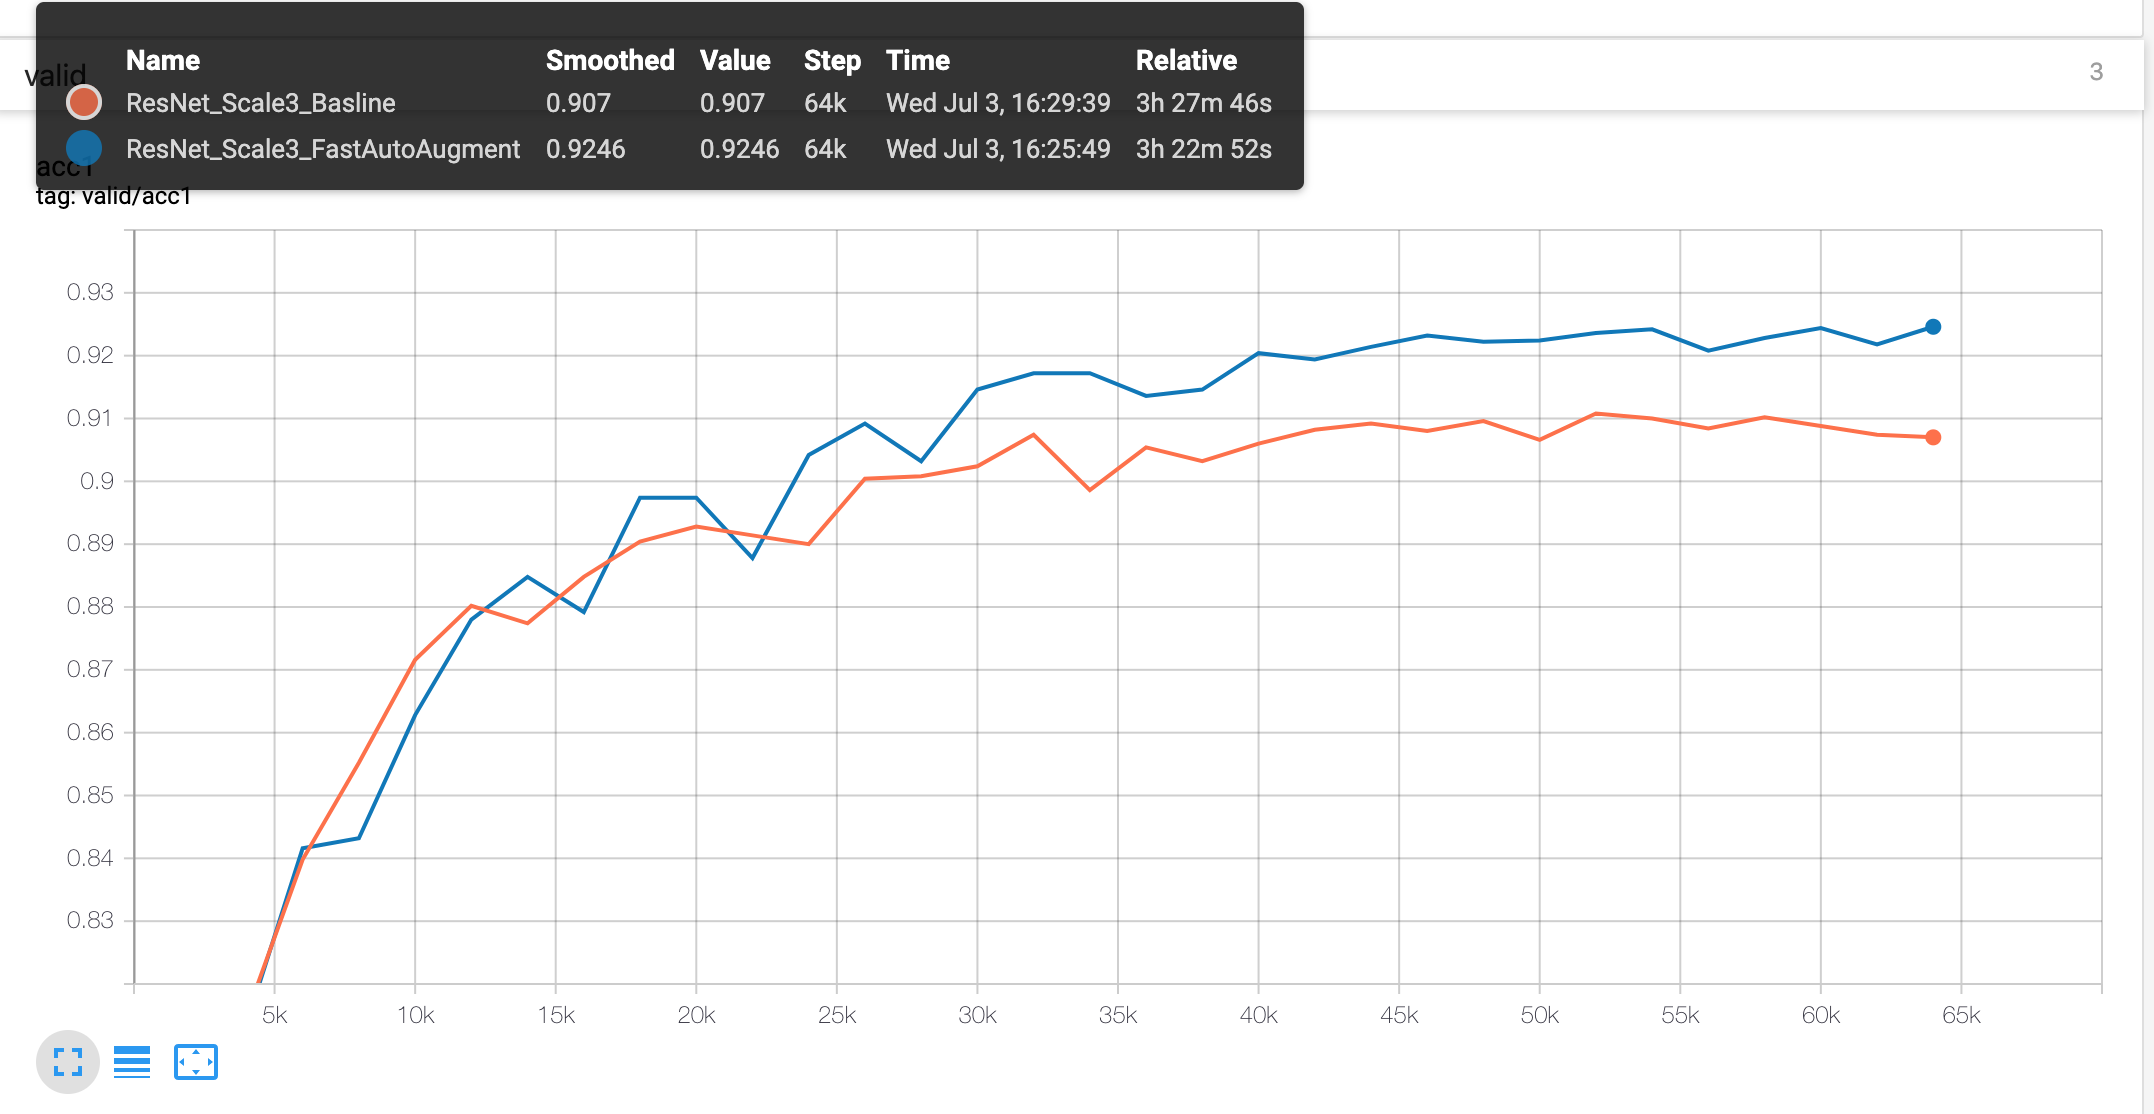
\includegraphics[width=\columnwidth]{resnet20_valid.png}
			\caption{FastAutoAugment Acc@1}
			\label{fig:FasetAutoAugment-accuracy}
		\end{center}
	\end{figure}

	\section{TDGA}
	\url{https://github.com/1g-hub/TDGA} にテンプレートレポジトリを作っておきました.最低限 pip で依存関係解消してインストールできるようにしたいと思ってます.
	ベースを deap でその中の selection 操作の 1 つとして拡張する形で作ろうと構想しているので,ほとんど書き方は deap のままで大丈夫になるはず.

	\section{来週のタスク}
	JSAI. TDGA 実装をすすめる.

	% 参考文献リスト
	\bibliographystyle{unsrt}
	\bibliography{2020_06_05}
\end{document}
